\documentclass{article}
\usepackage[utf8]{inputenc}
\usepackage[document]{ragged2e}
\usepackage{amsmath}
\usepackage{graphicx}
\usepackage{gensymb}
\usepackage[legalpaper, portrait, margin=1in]{geometry}
\graphicspath{ {./}}

\title{Lab 11 - Projectile Motion}
\author{\textbf{Corey Russ}\\\\Phys 222-03}
\date{Experiment Performed on 09/24/18}


\usepackage{natbib}
\usepackage{graphicx}

\begin{document}
\maketitle

\newpage
\section*{\begin{center}Abstract\end{center}}

When we conducted this experiment, we expected to be able to calculate the value for the initial velocity of a projectile launched from the Pasco launcher. We wanted to be able to correctly set up the launcher and gather precise data to allow us to calculate the initial velocity. We knew that we could obtain this value from the photogate attached to the launcher, but we wanted to be able to calculate it if we are able to find other quantities and relate some equations to each other. We measured our distances and angles to 1mm and 1$\degree$ respectively. Our experiment did not produce accurate results, as our measurements were not accurate.

\section*{\begin{center}Theory\end{center}}
Motion of projectiles can be viewed as parabolic. As a result, we can split the motion of projectiles into vertical and horizontal components. We can predict the initial launch velocity of a projectile if we are able to obtain the distance it travels, the height at which it was launched, and the angle it was launched at.
\subsection*{\begin{center}Horizontal Motion\end{center}}The horizontal component of projectile motion is simple. Assuming air resistance and friction are ignored, as well as a positive rightward direction, we can conclude from the following equation that the final horizontal velocity is equal to the initial horizontal velocity:\\\begin{center}Eq 1: $X_f = X_i+V_{ix}t+\frac{1}{2}a_xt^2$\end{center}
We know that the acceleration in the horizontal direction should be zero since no forces are acting in the horizontal direction as we are neglecting air resistance. In addition, our initial position is zero. Thus we can conclude the following:\\\begin{center}Eq 2: $X_f = V_{ix}t$\end{center}
\subsection*{\begin{center}Vertical Motion\end{center}}
The vertical component of projectile motion is similar to the horizontal. Assuming a positive upward direction:\\\begin{center}Eq 3: $Y_f = Y_i+V_{iy}t+\frac{1}{2}a_yt^2$\end{center}In our experiment $a_y = -g$, but our initial position is not zero. We now replace the acceleration into the equation and replace our final vertical position with zero:\\\begin{center}Eq 4: $0 = Y_i+V_{iy}t-\frac{1}{2}gt^2$\end{center}
\subsection*{\begin{center}Solving for Initial Vertical Velocity\end{center}}
To solve for the initial vertical velocity, we need to combine the two equations we have. Solving for time with the horizontal equation we obtain equation 5:\\\begin{center}Eq 5: $t = \frac{X_f}{V_icos\theta}$\end{center}We now substitute equation 5 for $t$ in equation 4 and obtain equation 6:\\\begin{center}Eq 6: $0 = Y_i+V_{i}sin\theta\frac{X_f}{V_icos\theta}-\frac{1}{2}g\frac{X_f^2}{V_i^2cos^2\theta}$\end{center}We now solve for $V_i$ and obtain equation 7:\\\begin{center}Eq 7: $V_i = \sqrt{\frac{gX_f^2}{2cos^2\theta(xtan\theta+Y_i)}}$\end{center}
\subsection*{\begin{center}Calculating uncertainty\end{center}}
Calculating the uncertainty is an important step in understanding our results. We need to be able to derive the uncertainty in our calculations to compare our data with theoretical data that includes slight errors in collecting measurements and data. To do this, we need the following equation:\\\begin{center}Eq 8: $\sqrt{\frac{g(x+\Delta x)^2}{2cos^2(\theta+\Delta\theta)[(x-\Delta x)(tan(\theta-\Delta\theta)+(Y_i-\Delta Y_i)]}}$
\end{center}
The $\Delta$ in equation 8 signifies the uncertainty in each value. Next, we take the result of equation 8 and apply it to equation 9 to obtain the uncertainty in $V_i$:\\\begin{center}Eq 9: $\Delta V_i = V_{i(max)}-V_{i(nominal)}$\end{center} Where $V_{i(nominal)}$ is the value that we calculate without taking into account the uncertainties.

\section*{\begin{center}Procedure\end{center}}
\subsection*{\begin{center}Equipment\end{center}}
The following items were necessary to collect our data:
\begin{itemize}
    \item Pasco MC 6800 Launcher and Photogate\\Used to launch and record the initial velocity of a projectile
    \item Computer with Pasco interface\\Used to gather launch data and export to Excel
    \item 2-Meter stick
    \item Carbon paper\\Used to record where the projectile landed
    \item Measuring calipers\\Used to measure the width of the projectile
\end{itemize}

\begin{figure}
\begin{center}
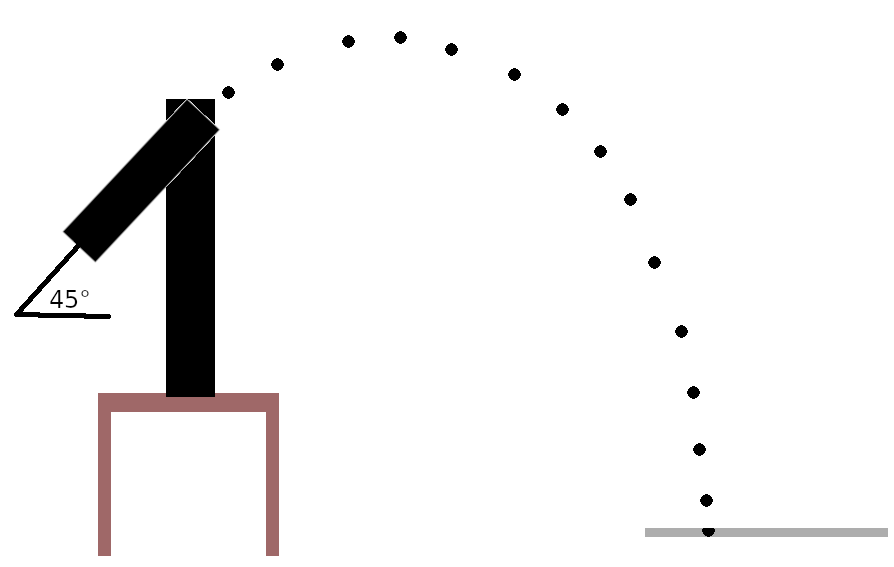
\includegraphics{1.png}
\caption{Setup}
\end{center}
\end{figure}


\subsection*{\begin{center}Collecting Data\end{center}}
We began setting up our equipment by placing the launcher on top of a chair. We measured the height of the chair and the projectile launcher and obtained a height of 0.865 meters. The angle of the Pasco launcher was set to $45\degree$, which was measured against a protractor on the launcher using a string and a weight attached to the launcher itself. We measured the width of the projectile using digital calipers and recorded an average reading of 0.02549 meters. Using our fingers, we pushed the projectile into the Pasco launcher until we reached the first click. To measure the final displacement of the projectile, we used a carbon paper to imprint the landing of the projectile. We used this spot and measured the distance from the launcher to this spot on the paper and obtained our displacements. We repeated this procedure to record different displacements and initial velocities.
\newpage
\section*{\begin{center}Data, Analysis, and Discussion\end{center}}

\subsection*{}
\begin{center}Table 1:\end{center}
\begin{center}
\begin{tabular}{|c|c|c|c|c|c|}
Angle($\degree)\pm1\degree$ & $Y_i(m)\pm1mm$ & $X_1(m)\pm1mm$ & $X_2(m)\pm1mm$ & $X_3(m)\pm1mm$ & $X_{avg}(m) \pm1mm$\\
45                    & 0.865         & 1.180         & 1.195         & 1.200         & 1.192                
\end{tabular}
\end{center}
\bigskip
We decided on the uncertainties of our measurements by using the smallest factor on the instrument. For example, the smallest measurement on the the 2-meter stick is 1mm, so that is what we chose. The same follows for the protractor on the Pasco launcher.

\subsection*{}
\begin{center}Table 2:\end{center}
\begin{center}
\begin{tabular}{|c|c|}
$V_i$ Photogate    & Speed ($\frac{m}{s}$) \\
1                  & 3.010                 \\
2                  & 3.010                 \\
3                  & 3.020                 \\
4                  & 3.020                 \\
5                  & 3.020                 \\
6                  & 3.020                 \\
7                  & 3.020                 \\
8                  & 3.000                 \\
9                  & 3.000                 \\
10                 & 2.990                 \\
Average            & 3.011                 \\
Standard Deviation & 0.011                
\end{tabular}
\end{center}

To calculate the initial velocity for the projectile, we used equation 7. We assume that $g$ is $9.8\frac{m}{s^2}$ downward. Substituting our data into equation 7 yields:
\begin{center}$V_{f(nominal)} = 2.6018\frac{m}{s}\approx\sqrt{\frac{9.8\frac{m}{s^2}\times(1.192m)^2}{2cos{^2}45\degree(1.192m\times tan45\degree+0.865m)}}$\end{center}

To calculate the uncertainty in our data, we used equation 8. Once again, we assume that $g$ is $9.8\frac{m}{s^2}$ downward. 
Using our data from Table 1, we substitute our values and the uncertainties we expected to find in our measurements:
\begin{center}$V_{f(uncertainty)} = 2.6787\frac{m}{s}\approx\sqrt{\frac{9.8\frac{m}{s^2}(1.192m+1mm)^2}{2cos^2(45\degree+1\degree)[(1.192m-1mm)(tan(45\degree-1\degree)+(0.865m-1mm)]}}$
\end{center}

$V_{f(uncertainty)}$ appears to be closer to the values we obtain for initial velocities using the Pasco computer software than $V_{f(nominal)}$. This indicates that we had significant errors in our measurements. When we compared $V_{f(nominal)}$ and $V_{avg}$ from Table 2, we found the percentage difference between the two values:
\begin{center}Difference $\% = \frac{V_{avg}-V_{f(nominal)}}{V_{avg}}\times 100$\end{center}
\begin{center}13.608 $\% = \frac{3.011\frac{m}{s}-2.6018\frac{m}{s}}{3.011\frac{m}{s}}\times 100$\end{center}
When we first looked at the percentage difference, we immediately saw that something was wrong. One of our first thoughts was that we took the measurements inaccurately. Our results are not able to conclude convincingly that we are able to estimate the initial velocity. We would have needed to take more accurate measurements and ensure that those measurements remained constant throughout the experiment to be able to verify our theory. Again, the discrepancy between our calculated $V_{f(nominal)}$ and $V_{avg}$ is too large be be conclusive.\\\medskip
There were many factors that contributed to this large discrepancy between the two velocities. We were unaware of it at the time, but perhaps the launcher itself was moved after each launch. We did not re-calibrate our system to accommodate for the change in position of the launcher. This would cause our displacement to either be larger or smaller depending on which direction the launcher moved. This would ultimately result in an inaccurate velocity. The second factor that would have skewed our results is an inaccurate setup of 45$\degree$. This would also change the range for our projectile and would also change the result calculated for our initial velocity. A possible reason for this is that we assumed the protractor attached to the Pasco launcher was accurate. Also, we assumed that the ground of the building was level, as well as the chair we placed the launcher on. We did not check the angle of the launcher after each launch. This would also provide false data since the angle could have been changed.


\section*{\begin{center}Conclusion\end{center}}

The primary objective of this experiment was to determine the initial launching velocity of a projectile shot from a Pasco launcher. After all of our measurements, we calculated an initial launching velocity. After this, we compared our velocity with the uncertainty in our velocity. We concluded from the results of these calculations that we did not complete the experiment correctly. This was primarily attributed to the fact that our measurements were not accurate. We did not control the system enough to ensure that our results would be conclusive.

\end{document}
